\documentclass{esannV2}
\usepackage[dvips]{graphicx}
\usepackage[latin1]{inputenc}
\usepackage{amssymb,amsmath,array}

\usepackage{xcolor}
\usepackage{hyperref}
\urlstyle{same}

%
\voffset 0 cm \hoffset 0 cm \addtolength{\textwidth}{0cm}
\addtolength{\textheight}{0cm}\addtolength{\leftmargin}{0cm}


\begin{document}
%style file for ESANN manuscripts
\title{A Study of Few-shot Learning on a Federated Setting}

%***********************************************************************
% AUTHORS INFORMATION AREA
%***********************************************************************

\author{Anna Mosolova$^1$, Elisa Lubrini$^1$ and Christophe Cerisara$^2$ 

% DO NOT MODIFY THE FOLLOWING '\vspace' ARGUMENT
\vspace{.3cm}\\
%
% Addresses and institutions (remove "1- " in case of a single institution)
1- Universite de Lorraine - IDMC \\
Pole Herbert Simon, 13 Rue Michel Ney, 54000 Nancy - France
%
% Remove the next three lines in case of a single institution
\vspace{.1cm}\\
2- Inria - \textcolor{green}{Dept of Second Author} \\
\textcolor{green}{Address of Second Author's school} - France\\
}
%***********************************************************************
% END OF AUTHORS INFORMATION AREA
%***********************************************************************

\maketitle

\begin{abstract}
Current restrictions on confidentiality often prevent data from leaving personal devices and being sent to central servers on which central models are trained. The problem of machine learning being hindered by scarcity of data can be tackled using few-shot learning (FSL) techniques. In this paper we explore the application of few-shot learning to a federated dataset, where each node (or device) only holds a limited amount of data. Our experiments are carried out using either an Induction Network, which leverages meta-learning to carry out classification tasks, or a pretrained BART model, by fine-tuning it to each node of the dataset.
\end{abstract}


%***********************************************************************


\section{Introduction}
Developing approaches to work with limited amount of data is becoming increasingly important, as legal restrictions make it harder and harder to access private data on personal devices.

Federated learning \cite{mcmahan2017communication}, a technique that has been raising in popularity since it was first introduced by Google in 2016, proposes a solution to the problem, allowing to train models on users' devices so that service providers can benefit from a model that has full access to private data, without the need for them to access such data directly.

Various architectures and methods are possible, both for the training of the single peripheral models and for merging the models into a single one. In this paper we want to propose the use of few-shot learning, a machine learning method used to generalise to a new task based on prior knowledge of other tasks \cite{wang2020generalizing}.

According to our knowledge, no experiments have been published so far applying few-shot learning to federated datasets and, given the timely relevance of finding optimal solutions to working with federated datasets, this paper aims to contribute to the field by reporting some of our related experiments.


%***********************************************************************


\section{Methodology}
Our experiments consist in the study of few-shot learning in a federated setting. Concretely, we use the Amazon Review dataset \cite{yu2018diverse} for sentiment analysis by distributing its data across a number of nodes (representing devices in a federated setting) each of which is then used to train a separate model.

We experiment with two different architectures: during a first experiment, each node will be trained using an Induction Network (IN) with meta-learning \cite{geng2019induction}, and in a second experiment the training will consist in fine-tuning pretrained BART models \cite{lewis2019bart}.

The reviews are divided in 23 categories according to the kind of product being reviewed. In order to accommodate the needs and limitations of each architecture, the dataset was distributed across the nodes in two different ways, for the training and test of: (1) the IN, and (2) the BART model. 

In each of the two experiments, once the models were trained they were used to instantiate two ensemble learning methods: averaging \cite{fedavg} and stacking \cite{wolpert}. The results were then compared to the corresponding baselines: the IN SoTA for the first experiment, and zero-shot \cite{zero} learning with BART models for the second experiment. 

    \subsection{Induction Networks}
    For the training, the samples were split into three sections, each of the three being assigned the reviews from 6 or 7 categories, as shown in Table \ref{tab:cats_in}. The remaining 4 categories were used for training.
        
    \setlength\parindent{24pt}
    \begin{table}[h!]
    \centering
    \hspace*{-50pt}\begin{tabular}{|c|c|c|}
    \hline
    Node & Ex. & Categories\\
    \hline
    1. & 23105 & apparel, office products, automotive, toys games, computer video games, software\\
    2. & 18146 & grocery, beauty, magazines, jewelry watches, sports outdoors, cell phones service, baby\\
    3. & 54333 & outdoor living, video, camera photo, health personal care, gourmet food, music\\
    \textit{Test} & \textit{120} & \textit{books, dvd, electronics, kitchen housewares}\\
    \hline
    \end{tabular}
    \caption{Portions of the dataset assigned to each node in the IN experiments.}\label{tab:cats_in}
    \end{table}
    
    We reused the implementation of the Induction Network by Zhongyu Chen\footnote{https://github.com/zhongyuchen/few-shot-text-classification}. After assigning to each node the relative categories (Table \ref{tab:cats_in}), each of the nodes was initialized as a separate model and trained only on the examples from the selected category. In order to combine the models and evaluate the resulting quality, we used averaging and stacking.
    
    The first one consisted in averaging the predicted probabilities from all models in order to obtain the final prediction. 
    
    For the stacking model we retrained the second node without the \textit{baby} category, so it has seen the examples only from the first 6 topics. Each model was then used to predict the probability distribution for the \textit{baby} domain. After this, they were used as features for training a meta-learner. As a meta-learner we tried several classical machine learning algorithms (Logistic Regression, Decision Trees and Support Vector Machines) as well as simple multi-layer perceptron. Usage of logistic regression as a meta-learner showed the best result which is reported in the next section.
    
    \subsection{BART} Since our BART model is pretrained, it is expected to produce good results with less examples, compared to the IN. For this reason, only the 4 categories previously used for testing (Table \ref{tab:cats_in}) were used, each to train a separate node with 30 examples (15 positive and 15 negative), as shown in Table \ref{tab:cats_b}.
        
    \begin{table}[h!]
    \centering
    \begin{tabular}{|c|c|c|}
    \hline
    Node & Ex. & Categories\\
    \hline
    1. & 30 & books\\
    2. & 30 & dvd\\
    3. & 30 & electronics\\
    4. & 30 & kitchen housewares\\
    \textit{Test} & \textit{120} & \textit{books, dvd, electronics, kitchen housewares}\\
    \hline
    \end{tabular}
    \caption{Portions of the dataset assigned to each node in the BART experiments.}\label{tab:cats_b}
    \end{table}
    
    First, we tried to evaluate the model without any training (Zero-shot learning setting), to use the results as a baseline. Subsequently, we fine-tuned 4 separate BART models using 3 support sets from the test data of the Amazon reviews dataset. We applied several combination methods on the resulting nodes. The first one was standard averaging consisting in averaging the probabilities from 4 models and outputting the results based on the final probabilities. The second one was weighted averaging that reused the previously described strategy but assigning to each node its own coefficient of contribution to the final prediction depending on its performance on the development set\footnote{The development set was constructed from 601 examples from the training set of the \textit{automative} domain.}. The third method was to apply the Federated Averaging strategy\cite{mcmahan2017communication} during the training of 4 nodes. This strategy consists in training models on separate nodes, then sending their weights to the server, averaging them and sending them back for a new round of training. 

        \begin{figure}[h!]
        \begin{center}
        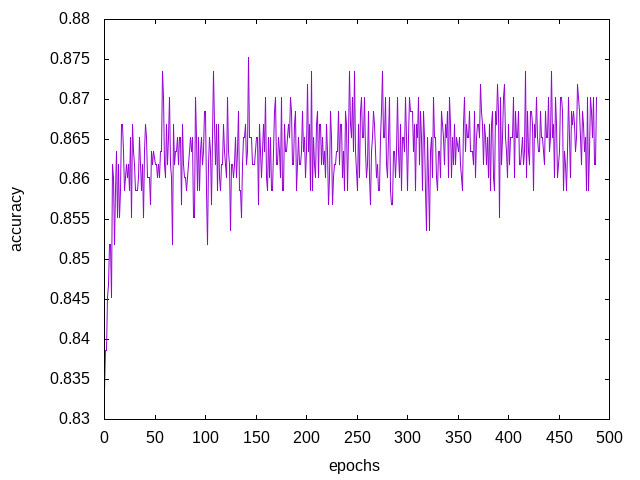
\includegraphics[width=8cm]{pics/dev.jpg}
        \caption[]{Evolution of the accuracy during fine-tuning on the development corpus.}
        \label{fig:dev}
        \end{center}
        \end{figure}


%***********************************************************************

        
    \section{Experiments}
        
        \subsection{Experimental Settings}
        \paragraph{Dataset} The dataset used for the experiments was the Amazon Review dataset from \cite{yu2018diverse}\footnote{The dataset is available at \url{https://github.com/Gorov/DiverseFewShot_Amazon}.}.
        For the BART experiments, each node was trained based on 3 labelling criterion (reviews from $n$ stars up being considered positive, with $n = 2$, $n = 4$, and $n = 5$), with each node being fine-tuned on 30 different examples, 10 per labelling criterion (5 positive and 5 negative).
        
        \paragraph{IN baseline} As a baseline, we used the original Induction Network introduced in \cite{geng2019induction} which was trained on the whole training set (19 domains). We compared its results with the results of the nodes which were the IN trained only on subparts of the original dataset. In addition to this, we evaluated their quality in a federated setting by averaging and stacking the predictions of the nodes.
        
        \paragraph{BART general settings} BART-MNLI-large\footnote{\url{https://huggingface.co/facebook/bart-large-mnli} (accessed on April, 1, 2021)} from HuggingFace, was used according to different settings: (1) Zero-shot one, (2) training on 12 support sets from the test data, (3) training 4 separate models on the support sets corresponding to one of the test domains and then combining them using several averaging strategies.
        
        \paragraph{weighted averaging} For weighted averaging we used the following coefficients: books - 0.1, dvd - 0.3, electronics - 0.4, kitchen housewares - 0.2 that were selected experimentally. The last one is training 4 BART nodes using Federated Averaging. 
        
        \paragraph{Hyper-parameters tuning}
        BART's hyper-parameters have been manually tuned with a few trials-and-errors
        on a development set extracted from the \textit{automotive} subset of the Amazon Reviews corpus.
        The development set is composed of 30 sentences for fine-tuning, and 600 sentences to compute the sentiment accuracy obtained with the fine-tuned BART-MNLI-large model.
        
        We have tried three fine-tuning strategies: (1) fine-tuning the full BART model, (2) fine-tuning only the first self-attention layer, (3) fine-tuning the inputs, outputs and layer normalization, following~\cite{}.
        
        The best hyper-parameters were achieved by fine-tuning all BART parameters, with a learning rate of $\lambda = 10^{-4}$ and 100 epochs. Figure~\ref{fig:dev} shows the evolution of the accuracy on the 600 development sentences during fine-tuning. We can observe that there does not seem to be any overfitting and that the performances plateau after epoch 100.
        
    \subsection{Experimental Results}
    Table \ref{Tab:induction_results} shows the results of all the Induction Network applications including the original one the results of which were reproduced using the implementation by Zhongyu Chen\footnote{https://github.com/zhongyuchen/few-shot-text-classification}.
    
        \begin{table}[h!]
      \centering
      \begin{tabular}{|c|c|}
        \hline
        Model & Mean Accuracy (\%) \\
        \hline
        Node 1 & 83.5 \\
        Node 2 & 83.3 \\
        Node 3 & 83.1 \\
        Averaging & 84.6 \\
        Stacking & 84.6 \\
        Reproduced model from \cite{geng2019induction} & 83.9 \\
        Result reported in \cite{geng2019induction} (SoTA) & 85.6 \\
        \hline
      \end{tabular}
      \caption{Results obtained with Induction Network from \cite{geng2019induction}.}\label{Tab:induction_results}
    \end{table}
    
    Table \ref{Tab:bart_results} shows the results obtained with the BART model (with and without fine-tuning). The values between parentheses give the standard deviation of the results after 5 trials.
    
    TODO: report statistical confidence interval at 90\% (look for Wald test):
    $$\pm 1.96 \sqrt{\frac {p(1-p)}{n=9000}}$$
    

    \begin{table}[h!]
      \centering
      \hspace*{-40pt}\begin{tabular}{|c|c|c|c|c|c|}
        \hline
        Model & Mean accuracy & Books & DVD & Electronics & KH \\
        \hline
        Zero-Shot Learning & 83.0 & 82.7 & 80.2 & 84.3 & 84.8 \\
        Books node & 85.1[$\pm 0.23$] & 86.4[$\pm 0.2$] & 83.4[$\pm 0.29$] & 85.0[$\pm 0.23$] & 85.3[$\pm 0.33]$ \\
        Dvd node & 85.2[$\pm 0.11$] & 86.8[$\pm 0.1$] & 83.9[$\pm 0.34$] & 85.0[$\pm 0.22$] & 85.5[$\pm 0.29$]  \\
        Electronics node & 84.4[$\pm 0.39$] & 84.4[$\pm 0.87$] & 82.1[$\pm 0.68$] & 85.3[$\pm 0.23$] & 86.1[$\pm 0.15$] \\
        Kitchen housewares node & 85.6[$\pm 0.12$] & 86.5[$\pm 0.22$] & 84.8[$\pm 0.37$] & 85.2[$\pm 0.22$] & 86.2[$\pm 0.17$]  \\
        Averaging of 4 nodes & 85.9 & 81.5 & 84.6 & 86.2 & 85.9  \\
        Weighted averaging & - & 86.8 & 84.4 & 86.0 & -  \\
        Federated Averaging & 85.7 & 86.7 & 84.4 & 85.7 & 86.0  \\
        \hline
      \end{tabular}
      \caption{Results obtained with BART.}\label{Tab:bart_results}
    \end{table}
    
    

%***********************************************************************



    \section{Conclusion}
    In this paper we have explored the combination of few-shot learning (FSL) and federated learning, which is currently a relevant topic given the increasingly rigid restriction on data protection, since a federated setting simulates the scarcity of data and few-shot learning allows for this scarcity not to be a hindrance.
    
    We explore this possible setting through two main experimental procedures, one by training Induction Networks through meta-learning, and one by fine-tuning BART models, on the task Sentiment Analysis.
    
    We showed that by applying FSL, we could obtain on a federated setting, results that are close to the current SoTA trained on a whole dataset. 

% ****************************************************************************
% BIBLIOGRAPHY AREA
% ****************************************************************************

\begin{footnotesize}

\bibliographystyle{unsrt}
\bibliography{bib.bib}

\end{footnotesize}

%\documentclass{esannV2}
\usepackage[dvips]{graphicx}
\usepackage[latin1]{inputenc}
\usepackage{amssymb,amsmath,array}

\usepackage{hyperref}
\urlstyle{same}

%***********************************************************************
% !!!! IMPORTANT NOTICE ON TEXT MARGINS !!!!!
%***********************************************************************
%
% Please avoid using DVI2PDF or PS2PDF converters: some undesired
% shifting/scaling may occur when using these programs
% It is strongly recommended to use the DVIPS converters, and to submit
% PS file. You may submit a PDF file if and only if you use ADOBE ACROBAT
% to convert your PS file to PDF.
%
% Check that you have set the paper size to A4 (and NOT to letter) in your
% dvi2ps converter, in Adobe Acrobat if you use it, and in any printer driver
% that you could use.  You also have to disable the 'scale to fit paper' option
% of your printer driver.
%
% In any case, please check carefully that the final size of the top and
% bottom margins is 5.2 cm and of the left and right margins is 4.4 cm.
% It is your responsibility to verify this important requirement.  If these margin requirements and not fulfilled at the end of your file generation process, please use the following commands to correct them.  Otherwise, please do not modify these commands.
%
\voffset 0 cm \hoffset 0 cm \addtolength{\textwidth}{0cm}
\addtolength{\textheight}{0cm}\addtolength{\leftmargin}{0cm}

%***********************************************************************
% !!!! USE OF THE esannV2 LaTeX STYLE FILE !!!!!
%***********************************************************************
%
% Some commands are inserted in the following .tex example file.  Therefore to
% set up your ESANN submission, please use this file and modify it to insert
% your text, rather than staring from a blank .tex file.  In this way, you will
% have the commands inserted in the right place.

\begin{document}
%style file for ESANN manuscripts
\title{Few-shot on Federated Learning}

%***********************************************************************
% AUTHORS INFORMATION AREA
%***********************************************************************

\author{Anna Mosolova$^1$, Elisa Lubrini$^1$ and Christophe Cerisara$^2$ 

%
% Optional short acknowledgment: remove next line if non-needed
%\thanks{This is an optional funding source acknowledgement.}
%
% DO NOT MODIFY THE FOLLOWING '\vspace' ARGUMENT
\vspace{.3cm}\\
%
% Addresses and institutions (remove "1- " in case of a single institution)
1- Universite de Lorraine - IDMC \\
Pole Herbert Simon, 13 Rue Michel Ney, 54000 Nancy - France
%
% Remove the next three lines in case of a single institution
\vspace{.1cm}\\
2- Inria - Dept of Second Author \\
Address of Second Author's school - France\\
}
%***********************************************************************
% END OF AUTHORS INFORMATION AREA
%***********************************************************************

\maketitle

\begin{abstract}
Current restrictions on confidentiality often prevent data from leaving personal devices and being sent to a central server on which a central model is trained. The problem of machine learning being hindered by scarcity of data can be tackled using few-shot learning (FSL) techniques. In this paper we explore the a possible application of few-shot learning to a federated dataset, where each node (or device) only holds a very limited amount of data. Our experiments are carried out using the T5 model, ......... The results of a few experiments are reported, together with a brief summary of our findings.
\end{abstract}

\section{Typesetting an ESANN document using \LaTeX}

This is a sample file. Please use this file to correctly typeset a
submission to the ESANN conference. The associated pdf file will
help you to have an idea of what your paper should look like.

\subsection{Page format and margins}
Please avoid using DVI2PDF or PS2PDF converters: some undesired
shifting/scaling may occur when using these programs
It is strongly recommended to use the DVIPS converters, and to submit
PS file. You may submit a PDF file if and only if you use ADOBE ACROBAT
to convert your PS file to PDF.
%
Check that you have set the paper size to A4 (and NOT to letter) in your
dvi2ps converter, in Adobe Acrobat if you use it, and in any printer driver
that you could use.  You also have to disable the 'scale to fit paper' option
of your printer driver.
%
In any case, please check carefully that the final size of the top and
bottom margins is 5.2 cm and of the left and right margins is 4.4 cm.
%t is your responsibility to verify this important requirement.  If these margin requirements and not fulfilled at the end of your file generation process, please use the commands at the beginning of the ESANNV2.tex file to correct them.  Otherwise, please do not modify these commands.


\subsection{Additional packages and functions}

Update the sample file according to your text. You can add
packages or declare new \LaTeX\ functions if and only if there is no conflict between your packages and the esannV2.cls style file.

\subsection{Style information}

\subsubsection{Page numbers}
Please do not add page numbers to this style; page numbers will be added by the publisher.
\subsubsection{Page headings}
Do not add headings to your document.
\subsection{Mathematics}
You may include additional packages for typesetting
algorithms, mathematical formula or to define new operators and environments
if and only if there is no conflict with the esannV2.cls
file.

It is recommended to avoid the numbering of equations when not
necessary. When dealing with equation arrays, it could be
necessary to label several (in)equalities. You can do it using the
`$\backslash$stackrel' operator (see the ESANNV2.tex source file);
example:

\begin{eqnarray}
c&=&|d|+|e|\nonumber\\
&\stackrel{\text{(a)}}{=}&d+e\nonumber\\
&\stackrel{\text{(b)}}{\geq}&\sqrt{f}\enspace,
\end{eqnarray}
\noindent where the equality (a) results from the fact that both
$d$ and $e$ are positive while (b) comes from the definition of
$f$.

\subsection{Tables and figures}

Figure \ref{Fig:MV} shows an example of figure and related
caption.  Do not use too small symbols and lettering in your
figures.  Warning: your paper will be printed in black and white
in the proceedings.  You may insert color figures, but it is your
responsibility to check that they print correctly in black and
white.  The color version will be kept in the ESANN electronic
proceedings available on the web.

\begin{figure}[h!]
\centering
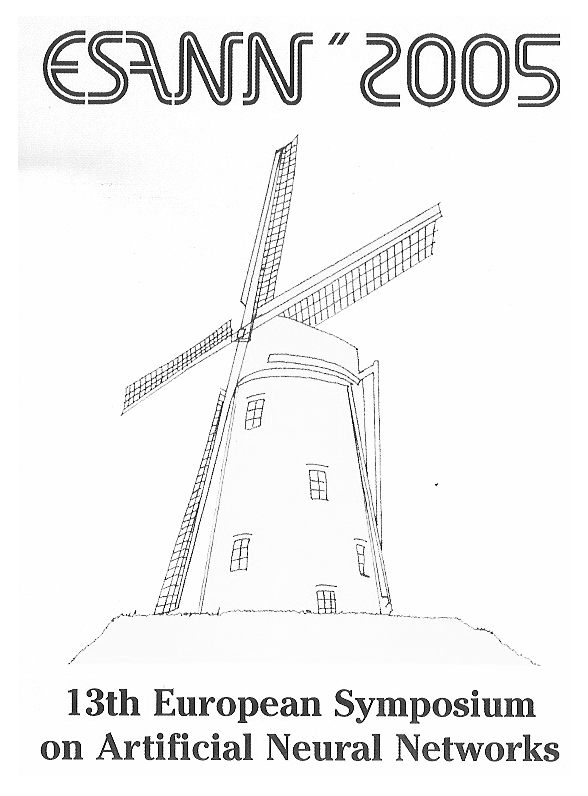
\includegraphics[scale=0.6]{ESANN2005BW.eps}
\caption{ESANN 2005: Announcement and call for
papers.}\label{Fig:MV}
\end{figure}

Table \ref{Tab:AgeWeight} shows an example of table.

\begin{table}[h!]
  \centering
  \begin{tabular}{|c|c|c|}
    \hline
    ID & age & weight \\
    \hline
    1& 15 & 65 \\
    2& 24 & 74\\
    3& 18 & 69 \\
    4& 32 & 78 \\
    \hline
  \end{tabular}
  \caption{Age and weight of people.}\label{Tab:AgeWeight}
\end{table}

\section{Citation}
This ESANNV2.tex file defines how to insert references, both for
BiBTeX and non-BiBTeX users.  Please read the instructions in this
file.

% ****************************************************************************
% BIBLIOGRAPHY AREA
% ****************************************************************************

\begin{footnotesize}

% IF YOU DO NOT USE BIBTEX, USE THE FOLLOWING SAMPLE SCHEME FOR THE REFERENCES
% ----------------------------------------------------------------------------
\begin{thebibliography}{99}

% For books
\bibitem{Haykin_book} S. Haykin, editor. \emph{Unsupervised Adaptive Filtering vol.1 : Blind Source Separation}, John Willey ans Sons, New York, 2000.

% For articles
\bibitem{DelfosseLoubaton_article}N. Delfosse and P. Loubaton, Adaptibe blind separation of sources: A deflation
approach, \emph{Signal Processing}, 45:59-83, Elsevier, 1995.

% For paper in proceedings published as serie books (LNCS,...)
\bibitem{CrucCichAmari_bookproceedings} S. Cruces, A. Cichocki and S. Amari, The minimum entropy and cumulants based contrast functions for blind source extraction. In J. Mira and A. Prieto, editors, proceedings of the 6$^{th}$ \emph{international workshop on artificial neural networks} ({IWANN} 2001), Lecture Notes in Computer Science 2085, pages 786-793,
Springer-Verlag, 2001.

% For paper in conference proceedings
\bibitem{VrinsArchambeau_proceedings} F. Vrins, C. Archambeau and M. Verleysen, Towards a local separation performances estimator using common ICA contrast functions? In M. Verleysen, editor, \emph{proceedings of the $12^{th}$
European Symposium on Artificial Neural Networks} ({ESANN} 2004),
d-side pub., pages 211-216, April 28-30, Bruges (Belgium), 2004.

% For Technical Report
\bibitem{Stone_TechRep} J. V. Stone and J. Porrill, Undercomplete independent component analysis for signal separation and dimension
reduction. Technical Report, Psychology Department, Sheffield
University, Sheffield, S10 2UR, England, October 1997.
\end{thebibliography}
% ----------------------------------------------------------------------------

% IF YOU USE BIBTEX,
% - DELETE THE TEXT BETWEEN THE TWO ABOVE DASHED LINES
% - UNCOMMENT THE NEXT TWO LINES AND REPLACE 'Name_Of_Your_BibFile'

\bibliographystyle{unsrt}
\bibliography{Name_Of_Your_BibFile}

\end{footnotesize}

% ****************************************************************************
% END OF BIBLIOGRAPHY AREA
% ****************************************************************************
\end{document}

\begin{table}[h!]
  \centering
  \begin{tabular}{|c|c|c|c|c|c|}
    \hline
    Training & Mean accuracy (\%) & Books & DVD & Electronics & KH \\
    \hline
    Books.t2 & 91 & 92 &  \\
    Books.t4 & 94 \\
    Books.t5 & 73 \\
    Dvd.t2 & 84 \\
    Dvd.t4 & 92 \\
    Dvd.t5 & 74 \\
    Electronics.t2 & 89 \\
    Electronics.t4 & 91 \\
    Electronics.t5 & 77 \\
    Kitchen housewares.t2 & 87 \\
    Kitchen housewares.t4 & 93 \\
    Kitchen housewares.t5 & 78 \\
    \hline
  \end{tabular}
  \caption{Results obtained with BART after training on books domain.}\label{Tab:bart_books}
\end{table}

\begin{table}[h!]
  \centering
  \begin{tabular}{|c|c|}
    \hline
    Training & Mean accuracy (\%) \\
    \hline
    Books.t2 & 92 \\
    Books.t4 & 95 \\
    Books.t5 & 73 \\
    Dvd.t2 & 86 \\
    Dvd.t4 & 92 \\
    Dvd.t5 & 74 \\
    Electronics.t2 & 88 \\
    Electronics.t4 & 90 \\
    Electronics.t5 & 78 \\
    Kitchen housewares.t2 & 86 \\
    Kitchen housewares.t4 & 93 \\
    Kitchen housewares.t5 & 77 \\
    \hline
  \end{tabular}
  \caption{Results obtained with BART after training on dvd domain.}\label{Tab:bart_dvd}
\end{table}


\end{document}
